\section{Navigation} \label{s:navi}
For make it possible to navigate a drone indoor, there are obstacles which is needed to be considered. There are two types of obstacles, permanent and temporally. The permanent obstacles can be as the following; walls, ceiling, doors, windows and furniture. Temporary obstacles are real time objects. This mean it is necessary to avoid any collision with any humans and other objects, that can occur suddenly in front of the drone. The drone should be capable of detecting those obstacles, but in some situations it can be an advantage to navigate the drone indoor. 
\newline

The drone needs to have different sensors to detect the obstacles. Sensor that can be used in these situations are distance sensors. The drone need a minimum number of distance sensors to cover all the surroundings. 
\ref{fig:drone_sensor}.
\begin{figure}[H]
    \centering
    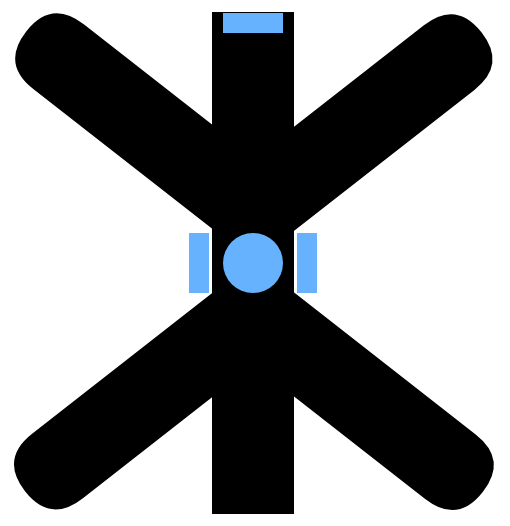
\includegraphics[width=0.3\textwidth]{figures/Navigation/DroneIR.png}
    \caption{Illustration of where the sensors are placed on the drone}
    \label{fig:drone_sensor}
\end{figure}
There are different sensors you can use to navigating a drone indoors. The following sensors which there will be a short description afterwards are:
\begin{itemize}
    \item Infra Red Sensor (IR sensor)
    \item Ultrasonic
    \item Vision sensor  
\end{itemize}
\subsection*{IR sensor}
One of the possible sensors are IR sensors, which is used in different devices such as laser distance meter. An IR sensor usually consist of an IR transmitter and an IR receiver. 
The IR sensor works by the transmitter sending an infrared light out, when the light hits an object, the light gets reflected back to the sensor's IR receiver. The distance then gets calculated from the time of flight, this is the time from when the light is sent out and to the sensor receives it again. This method is used to avoid collisions with obstacles, so the drone can keep a fixed distance to walls and ceilings.  
\newline
\newline
But there are some disadvantage with IR sensor, which could be light distortion, this could interfere with the sensor measuring. Another disadvantage is that the range is limited to 100-550 cm. 
\newline
Ultrasonic sensors works same as the IR sensors, but uses ultra sound instead. 

\subsection*{Vision sensor}\label{ss:camera_pa}
Vision sensors are sensors that consist of a camera, display, interface, and a computer processor. The way the sensor operates is by interchanging the data between the camera and a computer-based software. The following data, which in this case can be a video clip, will be processed first by the software and then it will be decided which actions should be taken. The software is already programmed with some desired criteria, such as distance measurement.
\newline
Vision sensors can be used in many tasks, here are some of the following tasks: 
\begin{itemize}
    \item High-speed product inspection (Quality control)
    \item Measurement
    \item Locating 
    \item Robot guidance 
\end{itemize}
The vision sensors can perform different taks and by the software identify shape, pattern, color, object detection including object gemotry and assembly and more.
%\begin{itemize}
   % \item Shape, pattern, or color
   % \item Object detection, including object geometry and assembly 
%\end{itemize}
However, there are some disadvantages to vision sensors, such as it can have difficulties to isolate the desired object in a congested environment. Another disadvantages is that it can have a high development costs in installation and training personnel in using it and difficult in maintining. 
%\begin{itemize}
  %  \item It can have difficulties to isolate the desired object in a congested environment
  %  \item High development costs in installation and training personnel
  %  \item Difficult in maintaining 
%\end{itemize}

From the problem analysis it can be concluded that, a time-of-flight sensor will suit this product the best. It is simple to implement and is also a good reliable sensor type. The only problem with it is the time it takes to have a distance, so it need a good sampling time, to make it possible to use it for checking the distance to a wall.
\newline
To make the sampling time as small as possible an IR-sensor is chosen, these type of sensors have a much quicker sampling time then a ultrasonic sensor, which use sound waves and the IR-sensor use light.
\newline
The IR-sensor VL53L0X will be used in the project, it is a time-of-flight sensor which uses IR light. 
\newline
\newline





